% Short papers (up to 4 pages) and long papers (up to 10 pages). 
% All submissions must be single-spaced double-column pages using 10-point size font on 8.5x11 inch pages (IEEE conference style),
% including figures, tables, and references.
\documentclass[conference]{IEEEtran}
\IEEEoverridecommandlockouts
% The preceding line is only needed to identify funding in the first footnote. If that is unneeded, please comment it out.
\usepackage{cite}
\usepackage{hyperref}
\usepackage{amsmath,amssymb,amsfonts}
\usepackage{algorithmic}
\usepackage{graphicx}
\usepackage{textcomp}
\usepackage[table]{xcolor}
\usepackage{multirow}

\def\BibTeX{{\rm B\kern-.05em{\sc i\kern-.025em b}\kern-.08em
    T\kern-.1667em\lower.7ex\hbox{E}\kern-.125emX}}
\begin{document}

\title{SPLA: Portable Generic Sparse Linear Algebra Library for Multi-GPU Computations\\
\thanks{Identify applicable funding agency here. If none, delete this.}
}

\author{\IEEEauthorblockN{1\textsuperscript{st} Egor Orachev}
\IEEEauthorblockA{\textit{Faculty of Mathematics and Mechanics} \\
\textit{St. Petersburg State University,}\\
\textit{Programming Languages and Tools Lab} \\
\textit{JetBrains Research}\\
St. Petersburg, Russia \\
egor.orachev@gmail.com\\
0000-0002-0424-4059}
\and
\IEEEauthorblockN{2\textsuperscript{nd} Gleb Marin}
\IEEEauthorblockA{\textit{School of Physics, Mathematics,} \\
\textit{and Computer Science} \\
\textit{HSE University}\\
St. Petersburg, Russia \\
glebmar2001@gmail.com\\
0000-0002-0873-1647}
\and
\IEEEauthorblockN{3\textsuperscript{rd} Semyon Grigorev}
\IEEEauthorblockA{\textit{Faculty of Mathematics and Mechanics} \\
\textit{St. Petersburg State University,}\\
\textit{Programming Languages and Tools Lab} \\
\textit{JetBrains Research}\\
St. Petersburg, Russia \\
s.v.grigoriev@spbu.ru\\
semyon.grigorev@jetbrains.com\\
0000-0002-7966-0698}
}

\maketitle

\begin{abstract}
    Scalable high-performance graph analysis is an actual nontrivial challenge and usage of sparse linear algebra operations as building blocks for graph analysis algorithms, which is a core idea of GraphBLAS standard, is a promising way to attack it.
    While it is known that sparse linear algebra operations can be efficiently implemented on GPGPU, full GraphBLAS implementation on GPGPU is a nontrivial task that is almost solved by GraphBLAST project. Though it is shown by GraphBLAST that utilization of GPGPUs for GraphBLAS implementation significantly improves performance, portability and scalability problems are not solved yet: GraphBLAST uses Nvidia stack and utilizes only one GPGPU.
    In this work we propose an SPLA library that aimed to solve these problems: it uses OpenCL to be portable and designed to utilize multiple GPGPUs.
    Preliminary evaluation shows that !!!!
\end{abstract}

\begin{IEEEkeywords}
graphs, algorithms, graph analysis, sparse linear algebra, GraphBLAS, GPGPU, OpenCL
\end{IEEEkeywords}

\section{Introduction}

Scalable high-performance graph analysis is an actual challenge.
There is a big number of ways to attack this challenge~\cite{Coimbra2021} and the first promising idea is to utilize general-purpose graphic processing units (GPGPU-s).
Such existing solutions, as CuSha~\cite{10.1145/2600212.2600227} and Gunrock~\cite{7967137} show that utilization of GPUs can improve the performance of graph analysis, moreover it is shown that solutions may be scaled to multi-GPU systems.
But low flexibility and high complexity of API are problems of these solutions.

The second promising thing which provides a user-friendly API for high-performance graph analysis algorithms creation is a GraphBLAS API~\cite{7761646} which provides linear algebra based building blocks to create graph analysis algorithms.
The idea of GraphBLAS is based on is a well-known fact that linear algebra operations can be efficiently implemented on parallel hardware.
Along with this, a graph can be natively represented using matrices: adjacency matrix, incidence matrix, etc.
While reference CPU-based implementation of GraphBLAS, SuiteSparse:GraphBLAS~\cite{10.1145/3322125}, demonstrates good performance in real-world tasks, GPU-based implementation is challenging.

One of the challenges in this way is that real data are often sparse, thus underlying matrices and vectors are also sparse, and, as a result, classical dense data structures and respective algorithms are inefficient. 
So, it is necessary to use advanced data structures and procedures to implement sparse linear algebra, but the efficient implementation of them on GPU is hard due to the irregularity of workload and data access patterns.
Though such well-known libraries as cuSparse show that sparse linear algebra operations can be efficiently implemented for GPGPU-s, it is not so trivial to implement GraphBLAS on GPGPU. 
First of all, it requires \textit{generic} sparse linear algebra, thus it is impossible just to reuse existing libraries which are almost all specified for operations over floats.
The second problem is specific optimizations, such as maskings fusion, which can not be natively implemented on top of existing kernels.
Nevertheless, there is a number of implementations of GraphBLAS on GPGPU, such as GraphBLAST:~\cite{yang2019graphblast}, GBTL~\cite{7529957}, which show that GPGPUs utilization can improve the performance of GraphBLAS-based graph analysis solutions.
But these solutions are not portable because they are based on Nvidia Cuda stack.
Moreover, the scalability problem is not solved: all these solutions support only single-GPU, not multi-GPU computations.

To provide portable GPU implementation of GraphBLAS API we developed a \textit{SPLA} library (sources are published on GitHub: \url{https://github.com/JetBrains-Research/spla}).
This library utilizes OpenCL for GPGPU computing to be portable across devices of different vendors.
Moreover, it is initially designed to utilize multiple GPGPUs to be scalable.
To sum up, the contribution of this work is the following.
\begin{itemize}
    \item Design of portable GPU GraphBLAS implementation proposed. The design involves the utilization of multipole GPUS. Additionally, the proposed design is aimed to simplify library tuning and wrappers for different high-level platforms and languages creation. 
    \item Subset of GraphBLAS API, including such operations as masking, matrix-matrix multiplication, matrix-matrix e-wise addition, is implemented. The current implementation is limited by COO and CSR matrix representation format and uses basic algorithms for some operations, but work in progress and more data formats will be supported and advanced algorithms will be implemented in the future.
    \item Preliminary evaluation on such algorithms as breadth-first search (BFS) and triangles counting (TC), and real-world graphs shows portability across different vendors and promising performance: for some problems Spla is comparable with GraphBLAST. Surprisingly, for some problems, the proposed solution on embedded Intel graphic card shows better performance than SuiteSparse:GraphBLAS on the same CPU. At the same time, the evaluation shows that further optimization is required.
\end{itemize} 
\section{Solution Description}

\subsection{Design Principles}

SPLA library is designed in the way to maximize potential library performance, to simplify its implementation and extensions, and to provided to the end-user verbose, but effective interface allowing customization and precise control over operations execution. This ideas are captured in the following principles.

\begin{itemize}
    \item \textit{DAG-based expressions}. User constructs a computational expression from basic nodes and uses oriented edges to describe data dependencies between these nodes. 
    \item \textit{Automated hybrid-storage format}. Library uses internally specialized preprocessing to format data and automate its sharing between computational nodes.
    \item \textit{Automated multi-GPU scheduling}. Computational work is automatically scheduled between available devices for execution. Scheduling order, dependencies and granularity are defined from DAG expression, submitted by user.
    \item \textit{Customization of primitive types and operations}. Underlying primitives types and functions, which operates on them, can be customized by user. Customization process does not requires library re-compilation. 
    \item \textit{Exportable interface}. Library has C++ interface with an automated reference-counting and with no-templates usage. It can be wrapped by C99 compatible API and exported to other languages, for example, in a form of a Python-package.
\end{itemize}

\subsection{Architecture Overview}

Library general execution architecture is depicted in Fig.~\ref{fig:architecture}. As an input library accepts expression composed in the form of a DAG.
Nodes represent fundamental operations, such as matrix-matrix multiplication. 
Links describe dependencies between nodes.
Expression execution is \textit{asynchronous}. 
User can block and wait until its completion, or without blocking probe the expression until it is either \textit{completed} or \textit{aborted}. 

Expression is transformed into a task graph. 
Task graph is submitted for execution to the task manager. 
Each task is processed by specialised \textit{NodeProcessor}, capable of processing particular node type.
Each task, when executed, is split dynamically into a set of parallel sub-tasks. 
Each sub-task is processed by specialized \textit{Algorithm}, which is capable of processing input blocks of matrices or vectors in particular storage formats with concrete set of options. \textit{NodePorcessor} and \textit{Algorithm} are selected at runtime from a registry of available set based on properties and arguments of the expression. 
Thus, it allows precise processing and optimization of edge-cases.

Granularity level of sub-tasks is defined by the structure of underlying processed primitives. 
Target device for execution is automatically assigned for the sub-task based on expression and node parameters. 
Currently, the uniform distribution for assignment is used, 
what should work good on large scale of computationally similar sub-tasks.

\begin{figure}[t]
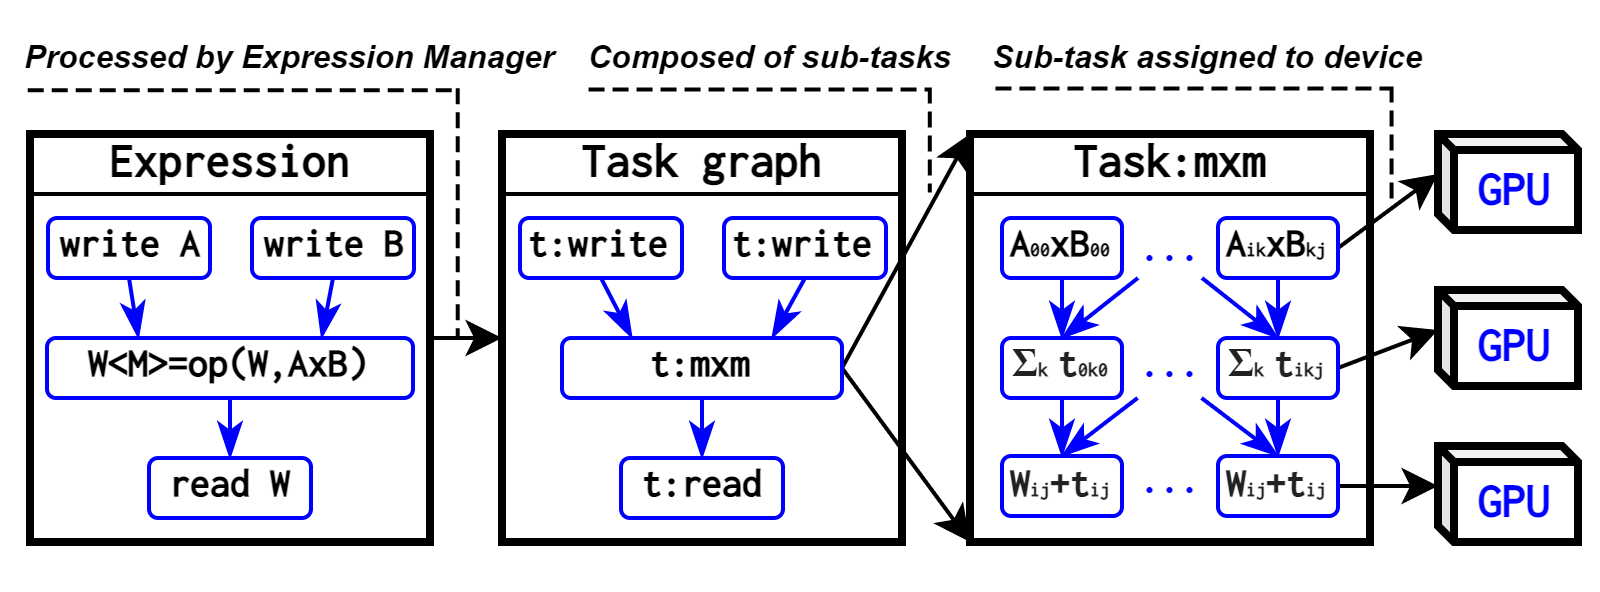
\includegraphics[width=0.99\linewidth]{figures/library_architecture.png}
\caption{Library expression processing architecture.}
\label{fig:architecture}
\end{figure}
    
\subsection{Matrices and Vectors}

Library provides general \textit{M-by-N Matrix} and \textit{N Vector} primitives.
Underlying primitives types is specified by \textit{Type} object. 
Internally primitives are stored in a hybrid storage in a form of two- or one- dimensional blocks' grid respectively. 
Each block is empty (not stored) or store some data in any format. Blocks are immutable, they can be safely shared across computational devices.

Currently only COO blocks are supported. Format choice is motivated by its simplicity and easy of implementation. 
Other formats, such as CSR, CSC, DCSR, Dense, etc. can be added to the library by either implementation of formats convertation or by the specialization of \textit{Algorithm} for concrete format.

\subsection{Algebraic Operations}

Library supports all commonly used linear algebra operations, such as \textit{mxm}, \textit{vxm}, \textit{eadd}, \textit{reduce}, \textit{transpose}. 
More operations coming later, since library still in development.
Interface of operations is designed in similar fashion as GraphBLAS ones. 
It supports \textit{masking}, \textit{accum} of the result, \textit{add} and/or \textit{mult} user-functions specification, and \textit{descriptor} object for additional operation tweaking.

\subsection{Implementation Details}

Library uses OpenCL 1.2 API as underlying compute API. 
Boost Compute~\cite{10.1145/2909437.2909454:boost:compute} is utilized as a high-level library on top of the OpenCL functionality. 
It provides thread-safe kernel caching, meta-kernel programming, and a set of basic parallel primitives such as \textit{device vector}, \textit{sort}, \textit{reduce}, \textit{scan}, etc. which was extended further to meet this project requirements.
Taskflow~\cite{Huang2022TaskflowAL} is used as tasking library. It supports task-dependencies and dynamic tasking, utilized in order to create and execute sub-tasks. 

User-defined \textit{Types} are represented as POD-structures, and handled by the library as a fixed-size sequences of bytes.
User-defined \textit{Functions} are effectively textual strings with OpenCL code, injected into generalized meta-kernels.
Library has a number of predefined types, such as \textit{signed/unsigned integers}, \textit{floating point} types, and a set of common operations, such as \textit{arithmetic}, \textit{logic}, \textit{first/second}, etc.

For particular blocked \textit{vxm} and \textit{mxm} \textit{Algorithms} implementations ESC algorithm~\cite{10.1145/2699470:esc:algo} for COO blocks is employed. 
Element-wise addition and masking are based on tiled GPU Merge Path~\cite{inproceedings:gpu_merge_path} algorithm. 
The code is generalized and is written in a form of meta-kernels, so actual functions for elements reduction or multiplication are injected later.
Kernel compilation is done on demand if no previously cached entry present.


\section{Evaluation}

For performance analysis of proposed solution we evaluated some most common graph algorithms using real-world sparse matrix data. 
As a baseline for comparison we chose LAGraph~\cite{szarnyas2021lagraph} in connection with SuiteSparse~\cite{10.1145/3322125} as a CPU tool, Gunrock~\cite{7967137} and GraphBLAST~\cite{yang2019graphblast} as a Nvidia GPU tools. 
Also, we tested algorithms on several devices with distinct OpenCL vendors in order to validate portability of the proposed solution. 
In general, these evaluation intentions are summarized in the following research questions. 

\vspace{0.2cm}
\begin{itemize}
    \item[\textbf{RQ1}] What is the performance of the proposed solution relative to existing tools for both CPU and GPU analysis?
    
    \item[\textbf{RQ2}] What is the portability of the proposed solution with respect to various device vendors and OpenCL runtimes?
\end{itemize}

\subsection{Evaluation Setup}

For evaluation, we use a PC with Ubuntu 20.04 installed, which has 3.40Hz Intel Core i7-6700 4-core CPU, DDR4 64Gb RAM, and Nvidia GeForce GTX 1070 GPU with 8Gb VRAM. 
Host programs were compiled with GCC 9.3.0 compiler. Programs using CUDA were compiled with GCC 8.4.0 and Nvidia NVCC 10.1.243 compiler.
Release mode and maximum optimization level was enabled for all tested programs. 
Data loading time, preparation, format transformations and host-device initial communications are excluded from time measurements. 
All tests are averaged across 10 runs.
Additional warm-up run for each test execution is excluded from measurements.

\subsection{Graph Algorithms}

For preliminary study \textit{breadth-first search} (bfs) and \textit{triangles counting} (tc) algorithms were chosen, since they allows analyse the performance of \textit{vxm} and \textit{mxm} operations, rely heavily on \textit{masking}, and utilize \textit{reduction} or \textit{assignment}. 
BFS implementation utilizes automated vector storage from sparse to dense switch and only \textit{}{push optimization}. 
TC implementation uses masked \textit{mxm} of source lower-triangular matrix with second transposed argument.

\subsection{Dataset}

Nine graph matrices were selected from the Sparse Matrix Collection at University of Florida~\cite{dataset:10.1145/2049662.2049663}. 
Information about graphs is summarized in Table~\ref{dataset:info}. 
All datasets are converted to undirected graphs. 
Self-loops and duplicated edges are removed.

\begin{table}[htbp]
\caption{Dataset description.} 
\begin{center}
    \rowcolors{2}{black!2}{black!10}
    \begin{tabular}{|l|r|r|r|}
    \hline
    Dataset & Vertices  & Edges & Max Degree \\
    \hline
    \hline
    coAuthorsCiteseer & 227.3K &   1.6M &    1372 \\
    coPapersDBLP      & 540.4K &  30.4M &    3299 \\
    hollywood-2009    &   1.1M & 113.8M &  11,467 \\
    roadNet-CA        &   1.9M &   5.5M &      12 \\
    com-Orkut         &     3M &   234M &   33313 \\
    cit-Patents       &   3.7M &  16.5M &     793 \\
    rgg\_n\_2\_22\_s0 &   4.1M &  60.7M &      36 \\
    soc-LiveJournal   &   4.8M &  68.9M &  20,333 \\
    indochina-2004    &   7.5M & 194.1M & 256,425 \\
    \hline
    \end{tabular}
    \label{dataset:info}
\end{center}
\end{table}

\subsection{Results}

Table~\ref{results} presents results of the evaluation and compares performance of Spla against other tool on different execution platforms.
Tools are grouped by the type of the device for the execution, where either Nvidia GPU or Intel CPU are used. 
Cell left empty if tested tool failed to analyse graph due to \textit{out of memory} exception.

In general, Spla BFS shows acceptable performance, especially on graphs with large vertex degree, such as soc-LiveJournal and com-Orkut.
On graphs roadNet-CA and rgg it has a significant performance drop due to the nature of underlying algorithms and data structures. 
Firstly, library utilizes immutable data buffers. Thus, iteratively updated dense vector of reached vertices must be copied for each modification, what dominates the performance of the library on a graph with large search depth. 
Secondly, Spla BFS does not utilise \textit{pull optimization}, what is critical in a graph with relatively small search frontier. 

Spla TC has a good performance on GPU, which is better in all cases that reference SuiteSparse solution. 
But in most tests GPU competitors, especially Gunrock, show smaller processing times. 
GraphBLAST shows better performance as well. 
Library utilises masked SpGEMM algorithm, the same as in GraphBLAST, but without \textit{identity} element to fill gaps. 
Library explicitly stores all non-zero elements, and uses mask to reduce only non-zero while evaluating dot products of rows and columns. 
What causes extra divergence inside work groups. 
On Intel device Spla shows better performance compared to SuiteSparse on com-Orkut, cit-Patents and soc-LiveJournal. 
A possible reason is the large lengths of processed rows and columns in the product of matrices.

Gunrock shows nearly best average performance due to its specialized and optimized algorithms.
Also, it has good time characteristics on a mentioned earlier roadNet-CA and rgg in BFS algortihm. 
GraphBLAST follows Gunrock and show good performance as well. 
But it runs out of memory on a two significantly large graphs con-Orkut and indochina-2004. 
Spla does not rut out of memory on any test due to simplified storage scheme.

\begin{table}[htbp]
\caption{Graph algorithms evaluation results.\\Time in milliseconds (lower is better).} 
\begin{center}
    \begin{tabular}{|l|r|r|r|r|r|}
    \hline
    \multirow{2}{*}{Dataset} & \multicolumn{3}{c|}{Nvidia} & \multicolumn{2}{c|}{Intel} \\
    \cline{2-6}
    & GR & GB & SP & SS & SP \\
    \hline
    \hline
    \multicolumn{6}{|c|}{BFS} \\
    \hline
    \rowcolor{black!10} hollywood-2009    &  20.3 &  82.3 &   36.9 &   23.7 &   303.4 \\
    \rowcolor{black!2 } roadNet-CA        &  33.4 & 130.8 & 1456.4 &  168.2 &   965.6 \\
    \rowcolor{black!10} soc-LiveJournal   &  60.9 &  80.6 &   90.6 &   75.2 &  1206.3 \\
    \rowcolor{black!2 } rgg\_n\_2\_22\_s0 &  98.7 & 414.9 & 4504.3 & 1215.7 & 15630.1 \\
    \rowcolor{black!10} com-Orkut         & 205.2 & -- -- &  117.9 &   43.2 &   903.6 \\
    \rowcolor{black!2 } indochina-2004    &  32.7 & -- -- &  199.6 &  227.1 &  2704.6 \\
    \hline
    \hline
    \multicolumn{6}{|c|}{TC} \\
    \hline
    \rowcolor{black!10} coAuthorsCiteseer &   2.1 &    2.0 &    9.5 &    17.5 &    64.9 \\
    \rowcolor{black!2 } coPapersDBLP      &   5.7 &   94.4 &  201.9 &   543.1 &  1537.8 \\
    \rowcolor{black!10} roadNet-CA        &  34.3 &    5.8 &   16.1 &    47.1 &   357.6 \\
    \rowcolor{black!2 } com-Orkut         & 218.1 & 1583.8 & 2407.4 & 23731.4 & 15049.5 \\
    \rowcolor{black!10} cit-Patents       &  49.7 &   52.9 &   90.6 &   698.3 &   684.1 \\
    \rowcolor{black!2 } soc-LiveJournal   &  69.1 &  449.6 &  673.9 &  4002.6 &  3823.9 \\
    \hline
    \hline
    \multicolumn{6}{l}{Tools: Gunrock (GR), GraphBLAST (GB), SuiteSparse (SS), Spla (SP).} \\
    \end{tabular}
    \label{results}
\end{center}
\end{table}
 
% Two GPU

% \begin{table}[htbp]
%     \caption{Table Type Styles}
%     \begin{center}
%     \begin{tabular}{|c|c|c|c|}
%     \hline
%     \textbf{Table}&\multicolumn{3}{|c|}{\textbf{Table Column Head}} \\
%     \cline{2-4} 
%     \textbf{Head} & \textbf{\textit{Table column subhead}}& \textbf{\textit{Subhead}}& \textbf{\textit{Subhead}} \\
%     \hline
%     copy& More table copy$^{\mathrm{a}}$& &  \\
%     \hline
%     \multicolumn{4}{l}{$^{\mathrm{a}}$Sample of a Table footnote.}
%     \end{tabular}
%     \label{tab2}
%     \end{center}
% \end{table}

\section{Conclusion}

In this paper we present a library for sparse Boolean linear algebra which implements such basic operations as matrix-matrix multiplication and element-wise matrix-matrix addition in both Cuda and OpenCL.
Evaluation shows that our Boolean-specific implementations faster and require less memory than generic, not the Boolean optimized, operations from state-of-the-art libraries. 
Thus, the specialization of operations for this data type makes sense. 

The first direction of the future work is to integrate all parts (OpenCL and Cuda backends) into a single library and improve its documentation and prepare to publish.
Moreover, it is necessary to extend the library with other operations, including matrix-vector operations, masking, and so on.
As a result a Python package should be published.

Another important step is to evaluate the library on different algorithms and devices.
Namely, algorithms for RPQ and CFPQ should be implemented and evaluated on related data sets.
Also, it is necessary to evaluate OpenCL version on FPGA which may require additional technical effort and code changes.

Finally, we plan to discuss with GraphBLAS community possible ways to use our library as a backend for GraphBLAST or SuiteSparse in case of Boolean computations.
Moreover, it may be possible to use implemented algorithms as a foundation for generalization to arbitrary semirings.


\bibliographystyle{IEEEtran}
\bibliography{spla_main}

\end{document}
